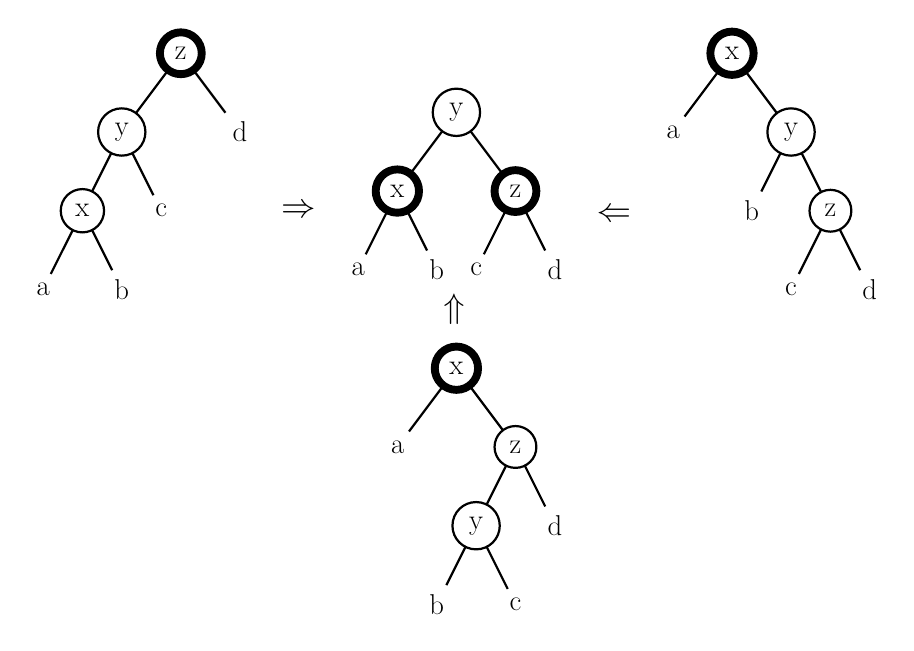
\begin{tikzpicture}[thick,scale=0.5, every node/.style={scale=0.5},level distance=2cm, sibling distance=2cm]
    \tikzstyle{tblack}=[circle, line width=1mm, draw=black]
    \tikzstyle{tred}=[circle, draw=black]
    \def\xstep{7cm}
    \def\ystep{8cm}
    
    \huge
    
%    % legend
%    \begin{scope}[xshift=7cm, yshift=7cm]
%        \def\inse{3.5mm}
%     %   \draw (-1, -2.5) rectangle (5, 1);
%        
%        \node[tblack, inner sep=\inse] at (0,0) {};
%        \node[tred, inner sep=\inse] at (0,-1.6) {};
%        \node[right=1pt] at (1,0) { -- черный};
%        \node[right=1pt] at (1,-1.6) { -- красный};
%    \end{scope}
    
%    \begin{scope}[yshift=\ystep]
%        \node[tblack] {z}
%            child { node[tred] {x}
%                child { node {a} }
%                child { node[tred] {y}
%                    child {node {b}}
%                    child {node {c}}
%                }
%            }
%            child { node {d} };
%    \end{scope}
    
    \begin{scope}[xshift=\xstep]
        \node[tblack] {x}
            child { node {a} }
            child { node[tred] {y}
                child { node {b} }
                child { node[tred] {z}
                    child {node {c}}
                    child {node {d}}
                }
            };
    \end{scope}
    
    \begin{scope}[xshift=-\xstep]
        \node[tblack] {z}
            child { node[tred] {y}
                child { node[tred] {x}
                    child {node {a}}
                    child {node {b}}
                }
                child { node {c} }
            }
            child { node {d} };
    \end{scope}
    
    \begin{scope}[yshift=-\ystep]
        \node[tblack] {x}
            child { node {a} }
            child { node[tred] {z}
                child { node[tred] {y}
                    child {node {b}}
                    child {node {c}}
                }
                child { node {d} }
            };
    \end{scope}
    
    \begin{scope}[yshift=-1.5cm]
        \tikzstyle{level 1}=[sibling distance=3cm]
        \tikzstyle{level 2}=[sibling distance=2cm]
        \node[tred] {y}
            child { node[tblack] {x}
                child { node {a} }
                child { node {b} }
            }
            child { node[tblack] {z}
                child { node {c} }
                child { node {d} }
            };
    \end{scope}
    \Huge
%    \draw (0, 0.5cm) node[rotate=-90] {$\Rightarrow$};
    \draw (0, -6.5cm) node[rotate=90] {$\Rightarrow$};
    \draw (-4cm, -4cm) node[rotate=0] {$\Rightarrow$};
    \draw (4cm, -4cm) node[rotate=180] {$\Rightarrow$};


    
\end{tikzpicture}
